\chapter{Regression}
As seen in the previous examples, regression analysis uses pre-existing data to understand the relationship between input features and the desired output. In regression analysis, there are five key terms that it's important to be familiar with.

\begin{itemize}
  \item The term \textbf{"Training data"} refers to the pre-existing data that includes the values of the desired output and the input features that affect the output.
  \item The term \textbf{"Target Variable"} refers to the feature of interest. In weather prediction, for example, the temperature would be the target variable. This variable is also sometimes referred to as the "dependent variable" because it is dependent on other variables.
  \item \textbf{"Independent Variables"} are those that are related to the target variable. The target variable often depends on multiple features, but each feature can have a different impact on the target variable. For example, in the case of temperature prediction, factors such as season, time, and regional geography all play a role, but each feature has a different level of influence on the temperature.
  \item \textbf{"Parameters}" refers to the coefficients that determine the relationship between the target variable and independent variables. Training a machine learning model involves identifying these parameters. The number of parameters depends on the complexity of the model.
  \item \textbf{"Residuals"}, also known as errors, refer to the discrepancy between the predicted and actual values.
\end{itemize}

Consider a retail company that utilizes Facebook ads to promote their products. The company wants to determine the effect of increasing their ad spending on their sales volume. In this example, the sales volume is the target variable ($y$) and the spending amount ($x$) is an independent feature. To examine the correlation between sales volume and spending amount, we first need to gather training data on past spending and sales. The relationship between spending and sales can be modeled using a linear equation $y = \omega_1 x + b$ or a polynomial equation $ y = \omega_1 x^k + \omega_2 x^{k-1} + \omega_3 x^{k-2}+ .. + b$. The goal of the machine learning model is to find the coefficients (parameters) that minimize the residual values (the difference between the actual and predicted values).

\newpage
\section{Linear Regression}

Linear Regression is a type of machine learning model that uses a linear equation to predict a target variable based on one or more independent variables. The goal is to find the best parameters that minimize the difference between the predicted and actual values.

It is a simple and widely used method, and can be further divided into simple and multiple linear regression based on the number of variables used.

\subsection{Simple Linear Regression}

Simple Linear Regression is a type of Linear Regression which models the relationship between one independent variable ($x$) and the target variable ($y$) using a linear equation as follow:
\begin{equation}\label{eq:lrmodel}
  y = \omega_1 x + b,
\end{equation} where the coefficient $\omega_1$ and cut off point $b$ are parameters that determine the linear equation used to model the relationship between the target and independent variable. Changing these parameters $\omega_1$ and $b$ results in different models that can describe the relationship between the target $y$ and independent variable $x$. For instance, using the $x$ and $y$ values in Table \ref{tb:lrmodel}, various linear equations can be formulated as below:
\begin{eqnarray}
% \nonumber to remove numbering (before each equation)
  y &=& 100x \\
  y &=& 100x + 800 \\
  y &=& 150x + 800 \\
  y &=& 125x + 800
\end{eqnarray}

\begin{table}[!ht]
\centering
\begin{tabular}{|c|c|c|c|c|c| }
  \hline
  $x$ & 0 & 1 & 2 & 3 & 4  \\
  \hline
  $y$ & 800 & 900& 100 & 1150 & 1300\\
  \hline
\end{tabular}
\caption{Example values of the target and the independent variable.}\label{tb:lrmodel}
\end{table}

The goal of a Simple Linear Regression model is to find the optimal parameters ($\omega_1$ and $b$) that can accurately predict the target variable ($y$)  for a new independent variable ($x$).

\begin{figure}[!h]
  \centering
  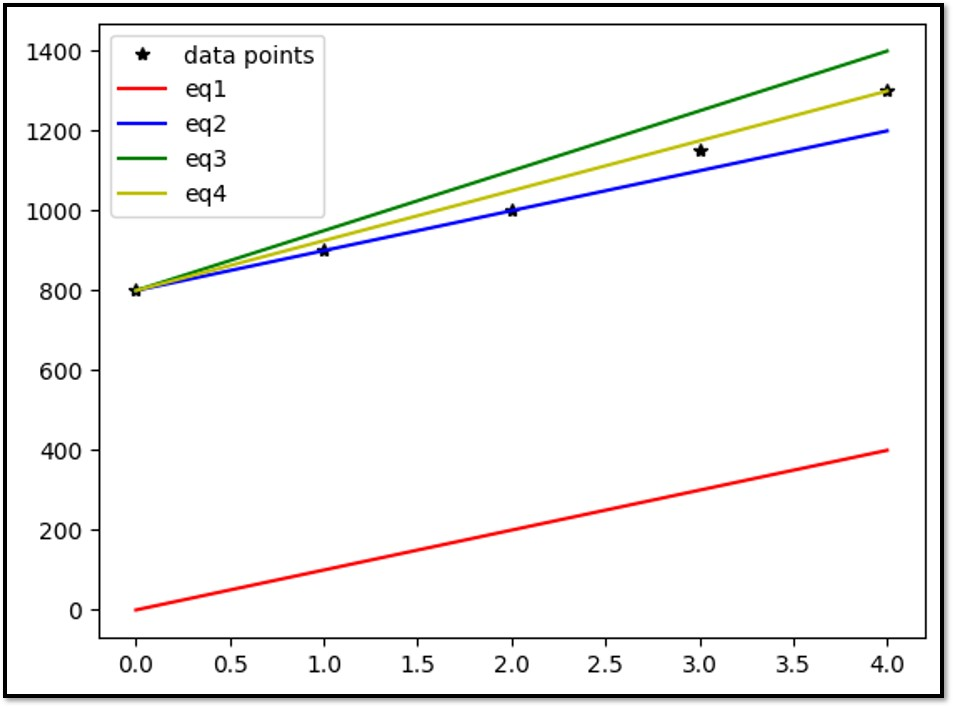
\includegraphics[width=8.2 cm]{LRmodel.jpg}
  \caption{An example of a Linear Regression Model}
  \label{fig:LRmodel}
\end{figure}

Figure \ref{fig:LRmodel} illustrates the data and the lines generated by the four different equations (2.2 to 2.5). The black stars represent the training data points listed in Table 2.1. It's clear that the red line does not fit the data points well and is not a good model. The yellow and blue lines pass through some of the data points. The goal of Simple Linear Regression is to find the parameters that produce a line that best describes the relationship between the target variable $y$ and independent variable $x$. The best model is the one that results in the least difference between the actual and predicted values.

\subsubsection{\textbf{Cost Function}}

The cost function is a measure of the average squared error (or residual) between the actual and predicted values. Mathematically,
\begin{equation}\label{eq:cost}
  \varepsilon = \frac{1}{N}\sum_{i=1}^N (\tilde{y_i}-y_i)^2,
\end{equation} where $N$ represents the number of data points (or observations) and $\tilde{y_i}$ represents the predicted value using the model, which can be described as:
\begin{equation}\label{eq:ypred}
   \tilde{y_i} = \omega_1 x_i + b,
\end{equation}where $\omega_1$ and $b$ are model parameters.

\newpage
\subsection{Multiple Linear Regression}
Multiple Linear Regression is an extension of Simple Linear Regression that takes into account more than one independent variable to predict the target value. This is achieved by using a linear equation, and it can be mathematically represented as:

\begin{equation}\label{eq:lrmodel}
  y = \omega_1 x_1 + \omega_2 x_2 + \omega_3 x_3 + ... + b,
\end{equation} where $\omega_i, i =0, 1, 2, ...$ are parameters of the model.

Like in Simple Linear Regression, the objective of Multiple Linear Regression is to find the parameters that minimize the cost function in equation \ref{eq:cost}. However, since it uses more than one feature, the different ranges of values of the features can lead to one feature having more influence than the other in predicting the target value. Therefore, it is essential to scale the features to have the same or similar ranges of values.

\newpage
\subsection{Feature Scaling}
Feature scaling is a technique used to adjust the independent variables to a similar range of values. There are several methods for feature scaling, including min-max scaling and z-score standardization, which are among the most widely used. Min-max scaling is often used in conjunction with neural networks, while z-score standardization is more frequently applied to linear regression models.

\subsubsection{\textbf{Min-Max Scaling}}
Min-max scaling, also referred to as normalization, is a method for scaling data into a range of 0 to 1. It is mathematically defined as:
\begin{equation}\label{eq:normalization}
   x_{scaled} = \frac{x-x_{min}}{x_{max}-x_{min}},
\end{equation}where $x_{min}$ and $x_{max}$ represent the minimum and maximum values of the variable $x$. The minimum value of $x$ will be mapped to 0 and the maximum value to 1, and all other values of $x$ will be scaled accordingly.

\newpage

\subsubsection{\textbf{Z-score Standardization}}
Z-score standardization, also known as zero-mean scaling, is a method that scales the values of each independent variable to have a mean of zero and a standard deviation of one. It can be calculated using the following formula:

\begin{equation}\label{eq:standardization}
   x_{scaled} = \frac{x-\mu}{\sigma},
\end{equation}where $\mu$ and $\sigma$ are mean and standard deviation of the variable $x$.

\newpage
\subsection{Assumptions}
There are four underlying assumptions in linear regression methods:
\begin{enumerate}
  \item \textbf{Linear relationship}: There should be a linear relationship between the target $y$ and independent variables $x_i$. This means that a change in $y$ due to a unit change in $x$  should be constant. If the relationship is not linear, the linear regression may not predict the target values correctly.
  \item \textbf{No multi-collinearity}: The independent variables should not be correlated, otherwise it becomes difficult to identify how they individually influence the target value and it can inflate the standard errors of some or all of the regression coefficients.
  \item \textbf{Consistent variance of residuals}: The variance of the residuals should be consistent across all predicted values, otherwise the estimates for the model coefficients may become unreliable.
  \item \textbf{Normally distributed residuals}: The residuals should be normally distributed, meaning most of the data points should be close to one straight line and the points farther away should fall off smoothly and symmetrically. If this is not the case, linear regression may not be a good choice for the problem.
\end{enumerate}

It is important to check if these assumptions are met when considering linear regression for modeling and deploying.

\newpage
\subsection{Knowledge Test}
\small{
\begin{questions} %<--- start option fixes number for first question
\question Table \ref{tb:lrmodel} shows the income earned by Mr 'Arm' based on the number of overtime hours he worked. Represent the relationship between the overtime hours and income using the equation $y=ax+b$ where $x$ represents overtime hours and $y$ represents income. Find the values of `a` and `b` and chose the best equation. Explain your reasoning for the chosen equation.
\begin{itemize}
  \item $y = 100 x + 800$
  \item $y = 125 x + 800$
  \item $y = 150 x + 800$
\end{itemize}
\question Why is feature scaling important in multiple linear regression?

\question What is the assumption of linearity in linear regression?

\question What is multi-correlation and why is it important to avoid in linear regression?

\question Can you explain the normality assumption in linear regression?

\question The multiple linear regression model for predicting sale volume is represented as $ y = 3.92 x_1 + 2.79 x_2 + 0.01x_3 + 14$ where $y$  is the sale volume, $x_1$  is the amount spent on TV advertising, $x_2$ is the amount spent on radio advertising, and $x_3$ is the amount spent on newspaper advertising.
\begin{enumerate}
  \item Which advertisement program has the least impact on sale volume? Can you explain your reasoning?
  \item If we increase the amount spent on TV advertising by one dollar while keeping the other two programs constant, what will be the resulting sale volume? Can you explain your reasoning?
\end{enumerate}

\end{questions}

\newpage
\section{Gradient Descent Method}\label{sec:GDS}
The Gradient Descent method is an optimization algorithm that finds the values of parameters (coefficients) that minimize a cost function. In the context of simple linear regression, the cost function depends on two parameters ($\omega_1$ and $b$) and can be represented in terms of the parameter $\theta$ as:

\begin{equation}\label{eq:costGDS}
  J(\theta) = \frac{1}{N} \sum_{i=1}^N \left((\omega_1 x_i + b) - y_i\right)^2,
\end{equation} where $\theta \in (\omega_1, b)$. To find the minimum of this function, we first compute the gradient, which measures the change in all weights in relation to the change in error. The changes of $J(\theta)$ with respect to $\omega_1$ and $b$ are given below as:

\begin{eqnarray}
  \frac{\partial J(\theta)}{\partial \omega_1} &=& \frac{2x_i}{N} \sum_{i=1}^N \left((\omega_1 x_i + b) - y_i\right)\\
  \frac{\partial J(\theta)}{\partial b} &=& \frac{2}{N} \sum_{i=1}^N \left((\omega_1 x_i + b) - y_i\right)
\end{eqnarray}

\newpage
\noindent The implementation of the Gradient Descent method can be broken down into four steps:

\begin{description}
  \item[Step 1] Initialize the parameters $\theta_k$.
  \item[Step 2] Compute the cost function value $J_k(\theta)$ using the parameters $\theta_k$.
  \item[Step 3] Update the parameters :
  \begin{equation}
  \theta_{k+1} = \theta_k - \alpha \frac{d J(\theta)}{d\theta}
  \end{equation} where the parameter $\alpha$ is a learning rate.
  \item[Step 4] Repeat steps 2 and 3 until the changes in cost function values are very small, or for a pre-defined number of iterations.
\end{description}

The performance of gradient descent is affected by the initial values of the parameters and the size of the learning rate. A high learning rate may prevent the algorithm from finding the local minimum and reaching the best solution, while a low learning rate may extend the time needed for the algorithm to reach convergence.

\begin{figure}[!h]
  \centering
  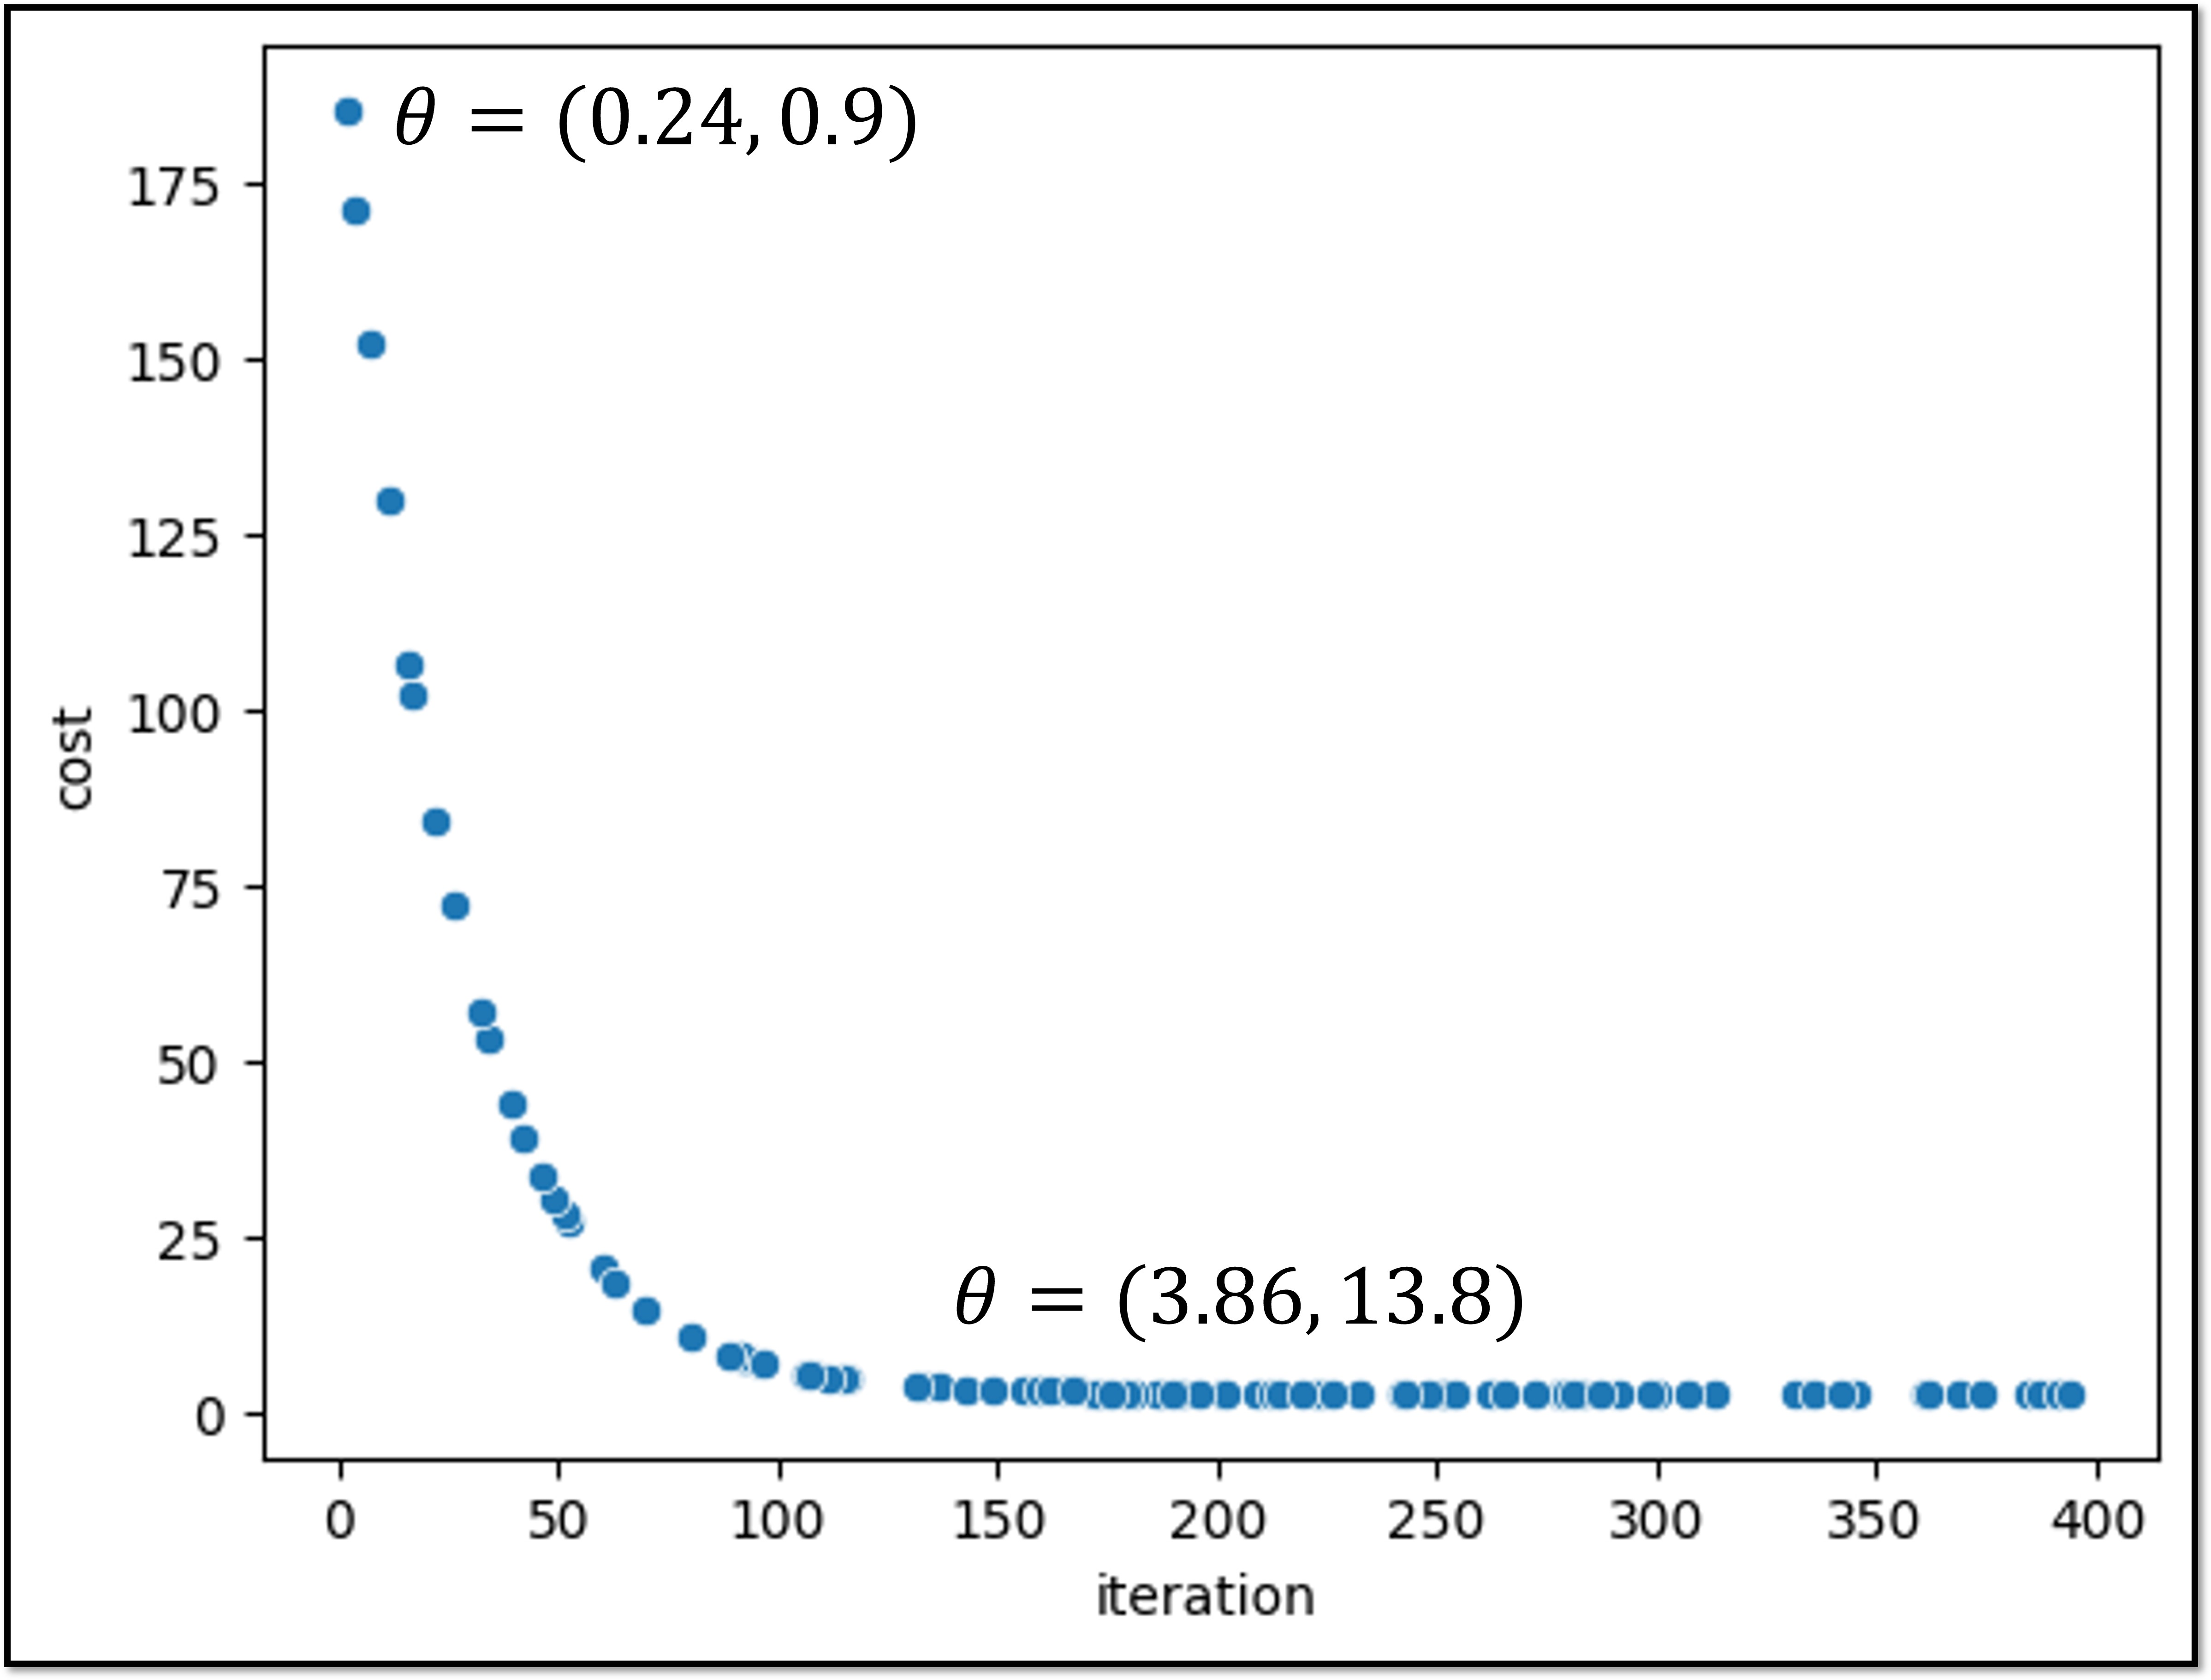
\includegraphics[width=7.5 cm]{gds_rate.jpg}
  \caption{How does the Gradient Decent Method work?}
  \label{fig:gdsRate}
\end{figure}

Figure \ref{fig:gdsRate} illustrates the operation of the gradient descent method. The parameter, $\omega_1$ and $b$ are initially set to $0.24$ and $0.9$ respectively. The gradient descent method then repeatedly modifies the parameters until the cost function reaches convergence. In this example, the cost function reaches a minimum value of $2.85$ at iteration 200, when the values of the parameters are $\omega_1 = 3.86$ and $b = 13.8$. Beyond iteration 200, the cost function does not change significantly, indicating that these values of the parameters provide the optimal solution with the smallest difference between the actual and predicted values.

\subsection{Knowledge Test}

\begin{questions}

\question Can you explain the concept of the learning rate in the gradient descent method?

\question What is the effect of feature scaling on the gradient descent method?

\question Figure \ref{fig:gdsRate} shows the values of cost function resulted by running gradient descent for 400 iterations with $\alpha =0.01$. The graph shows that the cost function, $J(\theta)$ decreases rapidly at first and then levels off.
\begin{itemize}
  \item what do you think will happen to the cost function if the learning rate is increased to 1 ($\alpha =1$)?
  \item what do you think will happen to the cost function if we decrease the value of the learning rate to 0.001 ($\alpha =0.001$)?
\end{itemize}

\end{questions}

\newpage

\section{Polynomial Regression}
A polynomial regression model represents the association between a target variable and one or more independent variables by means of an equation of the $n^{th}$ degree polynomial equation. When there is only one independent variable, $x$, the model can be formulated as

\begin{equation}\label{eq:polyEq}
  y = \omega_1 x^n + \omega_2 x^{n-1} + \omega_3 x^{n-2} + ... + \omega_n x + b
\end{equation} where $b$ is the cut off point, and $\omega_i$ where $i$ ranges from $1$ to $n$ are coefficients of the independent variable.


\begin{figure}[!ht]
  \centering
  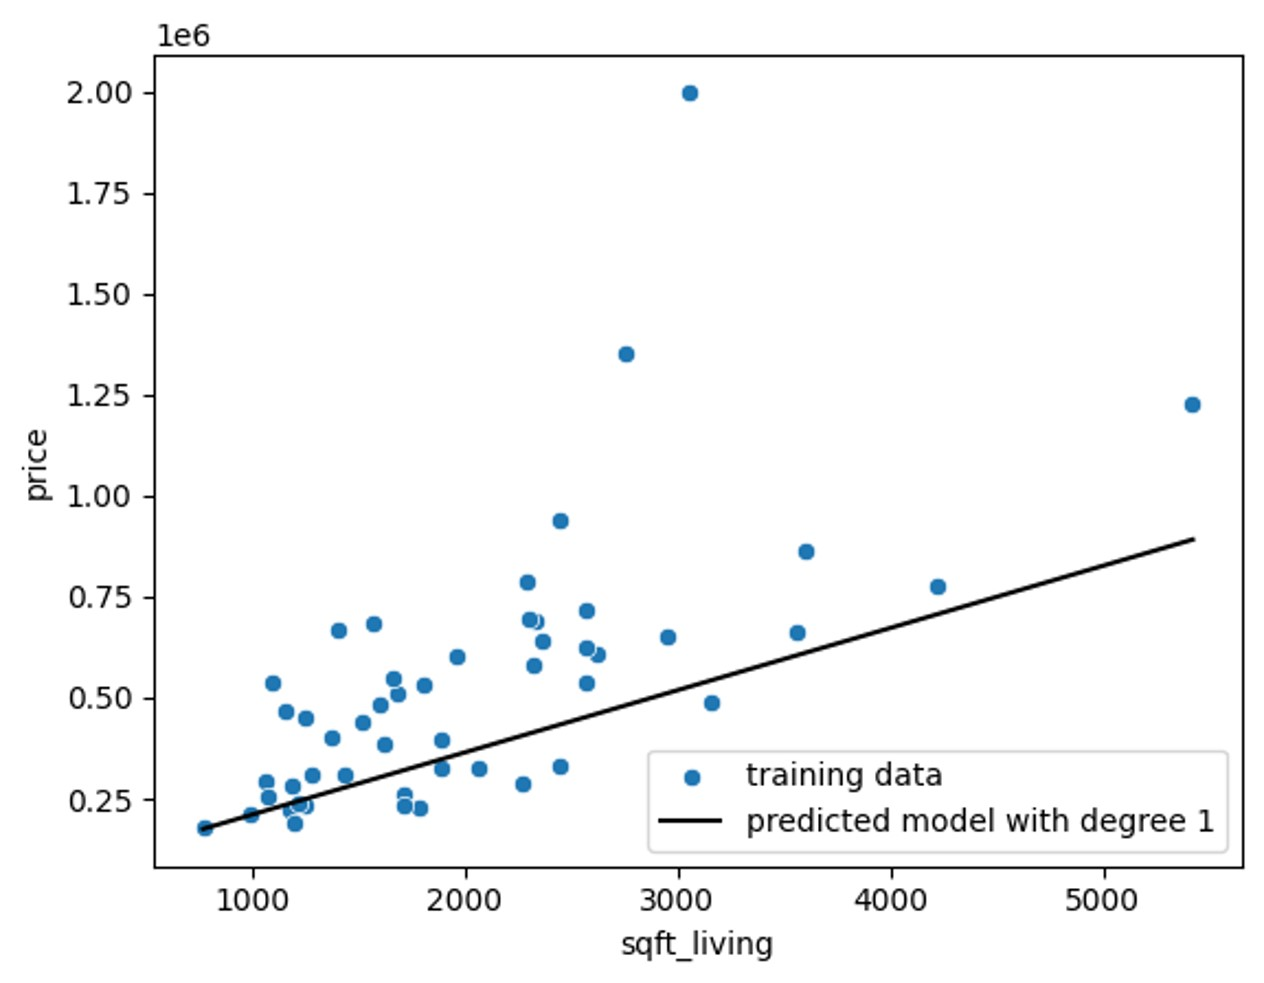
\includegraphics[width=4 cm]{poly_demo1.jpg}
  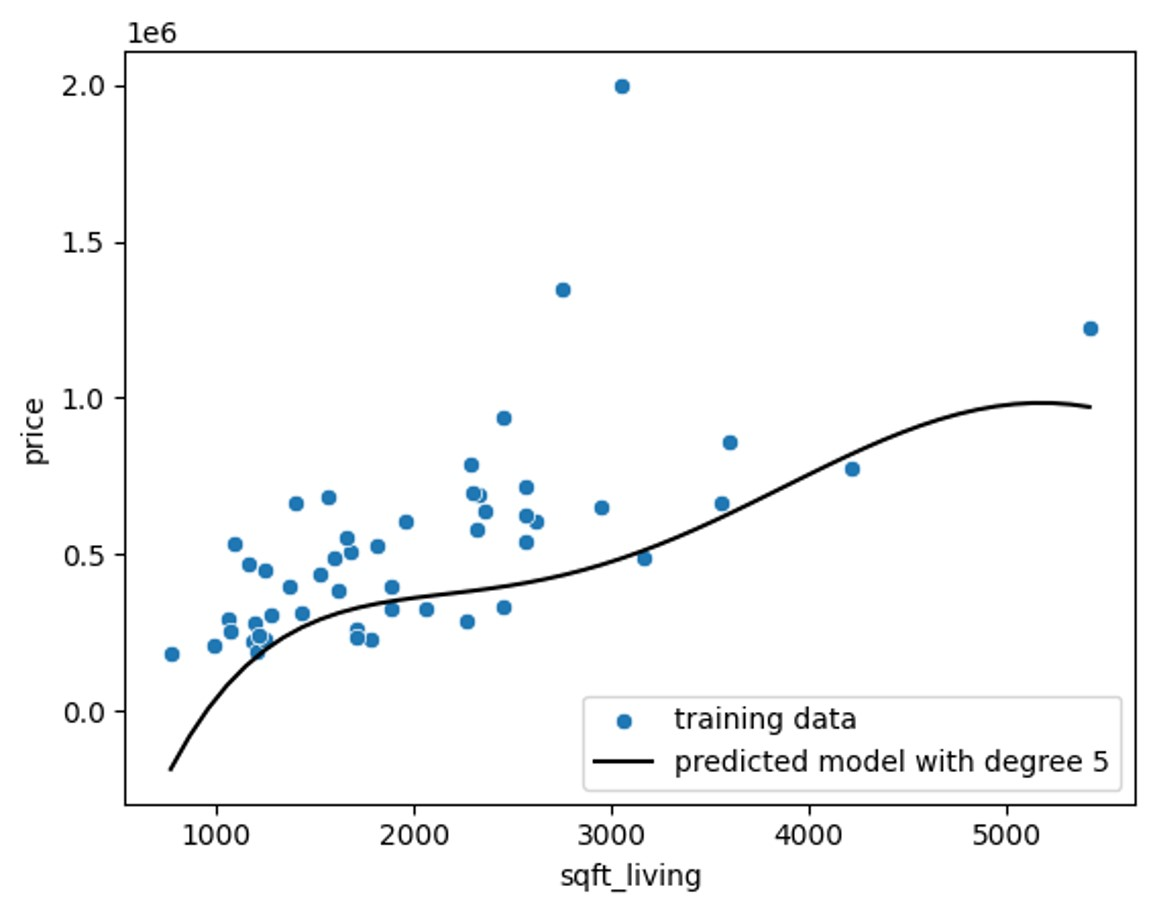
\includegraphics[width=4 cm]{poly_demo2.jpg}
  \caption{Linear Regression vs. Polynomial Regression}
  \label{fig:polydemo}
\end{figure}

Figure \ref{fig:polydemo} illustrates the difference between linear and polynomial regression when using a single feature. Polynomial regression uses a curve to fit the data, while linear regression uses a straight line. As the degree of the polynomial increases, the fit of the curve to the data improves and the difference between actual and predicted values decreases. In general, when the relationship between the target and independent variables is non-linear and cannot be represented by a straight line, polynomial regression tends to provide a better fit than linear regression.

However, using a higher degree polynomial also increases the number of parameters and makes the computation more complex. For a single feature, the number of parameters for an $n^{th}$ degree polynomial is $n+1$, and it would be even higher for multiple features.
\newpage
\subsection{Multiple Features}
The mathematical equation for a 2nd-order polynomial regression model with 2 independent variables is as follows:

\begin{eqnarray}\label{eq:MpolyEq}
% \nonumber % Remove numbering (before each equation)
\nonumber  y &=& \omega_1 x_1^2 + \omega_2 x_1 + \omega_3 x_2^2 + \omega_4 x_2 \\
             &+& \omega_5 x_1 x_2 + b
\end{eqnarray} A $2^{nd}$-order polynomial regression model with 4 features has 5 coefficients and one association and one cut-off point. As the polynomial degree and number of features increase, the number of coefficients also increases.

\newpage
\subsection{Implementation}
In contrast to linear regression methods, using polynomial regression requires an additional step, as illustrated in Figure \ref{fig:polyImple}. The data must be transformed to a higher dimensional space in order to model the relationship between the target and independent variables using a linear equation. Then, the parameters can be determined using the Gradient descent method, as previously described in section \ref{sec:GDS}.

\begin{figure}[!ht]
  \centering
  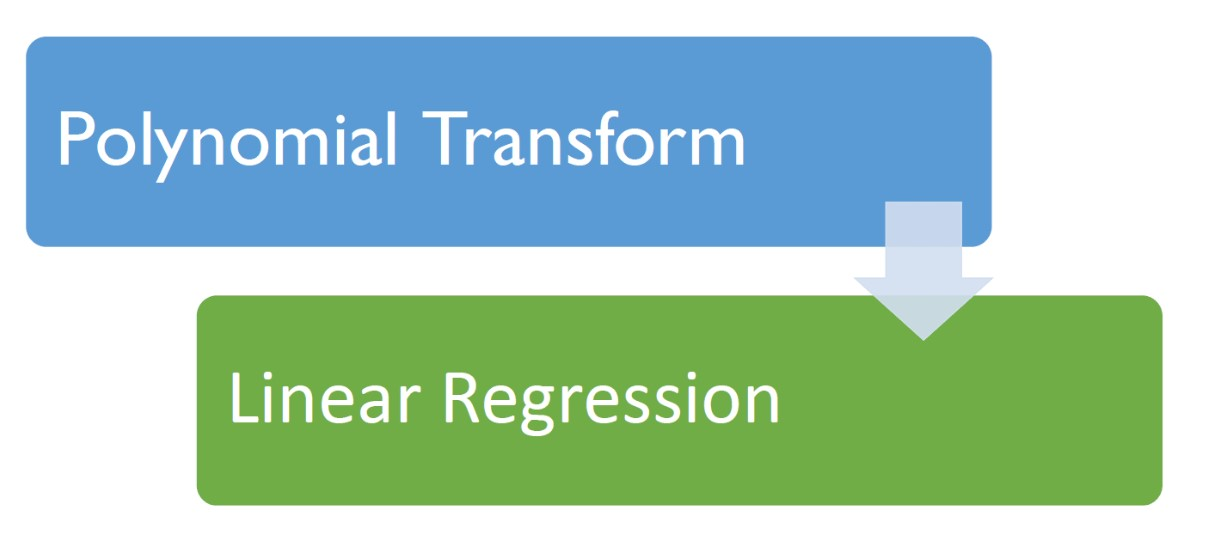
\includegraphics[width=6 cm]{poly_transform.jpg}
  \caption{Polynomial Regression Implementation}
  \label{fig:polyImple}
\end{figure}

\newpage
\subsection{Hyper-parameter}
In polynomial regression, the degree of order is a hyper-parameter that must be selected and provided as input to the model. Typically, a higher degree of order will provide a better fit to the data and result in a lower difference between actual and predicted values. However, as the order increases, the model may attempt to fit every single data point in the data-set and lose its ability to generalize to new data, known as over-fitting. The topic of how to prevent over-fitting and choose appropriate hyper-parameters will be discussed in section \ref{sec:hyperP}.

\newpage
\subsection{Knowledge Test}
\begin{questions}

\question How does polynomial regression differ from linear regression?

\begin{figure}[!h]
  \centering
  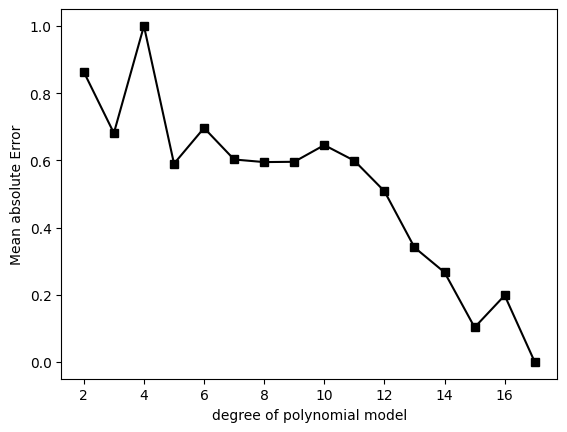
\includegraphics[width=6 cm]{order_poly.png}
  \caption{Mean squared error vs. order of the Polynomial regression Model}
  \label{fig:polyOrder}
\end{figure}

\question Figure \ref{fig:polyOrder} shows the plot of the mean squared error obtained for different order of the polynomial regression model. Which order of the polynomial regression model has the lowest mean squared error? Can you explain why this may or may not be the best choice?
\end{questions}

\newpage

\section{Model Implementation}\label{sec:model}
The implementation of machine learning models has become much simpler and more efficient with the advancement of various python libraries. This section will cover the step-by-step process of implementing a machine learning model using Python.

\subsection{Data Preparation}
Data preparation, also known as data pre-processing, is a necessary step before building any machine learning model. This stage includes:
\begin{itemize}
  \item cleaning the data, such as removing outliers and identifying incorrect or missing information,
  \item analyzing the data to understand the relationship between the target and different features, and detect any correlation among features,
  \item creating new features from the existing features through feature engineering.
\end{itemize}In summary, this stage makes the data suitable for use in the machine learning modeling process.


\newpage
\subsection{Data Splitting: Train-Test Split}
A supervised regression method aims to predict unseen data using a model trained on labeled data. If all of the available data is used to train the model and determine its parameters, the model may perform well on the training data but poorly on unseen data. To ensure the model will perform well on unseen data, it is important to set aside a portion of the data as a testing set.

The process of dividing the labeled data into a training set for model training and a testing set for evaluation is called Train-Test Split. To ensure that the model is accurate, it is crucial to use a sizable training set that captures the underlying correlations in the data, and to randomly select the data for the split to create representative sets. Usually, the standard practice is to use two-thirds of the data for training and the remaining one-third for testing.

\subsubsection{\textbf{Train-Test Split in Python}}
The scikit-learn library in Python makes it easy to perform data splitting using the train\_test$\_$split function from the model$\_$selection module. This function takes a loaded data-set as input and separates it into two subsets. It is a good practice to first separate the independent variables ($X$) and the target variable ($y$) from the labeled data, and then pass $X$ and $y$ to the train$\_$test$\_$split function. This function will randomly split both $X$ and $y$ into training and testing sets.

In the example provided, the data set used is "Advertising.csv" \cite{web:adData}, in which the sale amount is the target variable and depends on the advertisement cost in  \emph{`TV', `radio', and `newspaper'}. The below python codes read the \emph{`Advertising'} data set from the data folder and extract the independent variables ($X$) and the target variable ($y$) from the data-set. Then, the data set is randomly split into 67 percent as training and 33 percent as testing data.

\begin{lstlisting}[language=Python]
# ==================================================#
import pandas as pd
from sklearn.model_selection import train_test_split

df=pd.read_csv('..\\data\Advertising.csv')
X=df[['TV', 'radio', 'newspaper']]
y=df['sales']

X_train, X_test, y_train, y_test = train_test_split(X,y,
                                    test_size = 0.33,
                                    random_state=1)
# ==================================================#
\end{lstlisting}
The random state is set at 1 so that the same subset is provided by Python every time we run the code.

\newpage
\subsection{Data Modelling}
In this stage, a machine learning method is modeled using a training dataset. The section includes discussion and implementation of linear and polynomial regression using Python.

\subsubsection{\textbf{Linear Regression in Python}}
The following code demonstrates how to model linear regression using the Python sklearn library. It is important to note that the $X_{train}$ variable includes multiple features. The code for both simple and multiple linear regression is the same, except for the dimensions of the $X_{train}$ variable. The "\emph{fit}" function under the Linear Regression module finds the optimal parameters that minimize the difference between the actual and predicted values of the target variable, "sale amount."

\begin{lstlisting}[language=Python]
# ==================================================#
from sklearn.linear_model import LinearRegression

lr = LinearRegression()
lr.fit(X_train, y_train)

print(lr.coef_, lr.intercept_)

# ==================================================#
\end{lstlisting}

Feature scaling is a crucial step in building a multiple linear regression model. It can be accomplished by using the pre-processing module in the sklearn library.

The following Python code demonstrates how to perform feature scaling and then use the scaled features to train a linear regression model. By normalizing the features, it can make sure that one feature does not dominate over the other, and all the features are on the same scale, which can help the optimization algorithm converge faster. It can also help to prevent numerical instability and can improve the performance of the model.

\begin{lstlisting}[language=Python]
# ==================================================#
## feature scaling

from sklearn.preprocessing import StandardScaler

scale = StandardScaler()
X_scaled = scale.fit_transform(X_train)
## linear regression model
from sklearn.linear_model import LinearRegression

lr = LinearRegression()
lr.fit(X_scaled, y_train)
print(lr.coef_, lr.intercept_)
# ==================================================#
\end{lstlisting}


\subsubsection{\textbf{Polynomial Regression in Python}}

Polynomial regression is an extension of linear regression that involves a step of feature transformation. The following code demonstrates how to implement polynomial regression using the sklearn library. It is performed by adding polynomial features, which are derived from the original features, to the input data-set, and then fitting a linear model to the transformed data. This can help to capture non-linear relationships between the input and output variables, which linear regression cannot capture.

\begin{lstlisting}
# ==================================================#
## Poly regression model
from sklearn.preprocessing import PolynomialFeatures

poly = PolynomialFeatures(degree=5, include_bias=False)
X_poly = poly.fit_transform(X_scaled)

from sklearn.linear_model import LinearRegression
lr_poly = LinearRegression()
lr_poly.fit(X_poly, y_train)
# ==================================================#
\end{lstlisting}

The Polynomial Features module is utilized to transform the features into a $5^{th}$-order polynomial equation in a higher-dimensional linear space. This is done before performing linear regression on the transformed features. By increasing the number of dimensions in the feature space, it can allow the linear model to fit more complex and flexible decision boundaries, which can increase the model's ability to generalize to unseen data.
%----------------------
\subsubsection{\textbf{Pipeline}}
\begin{figure}[!h]
  \centering
  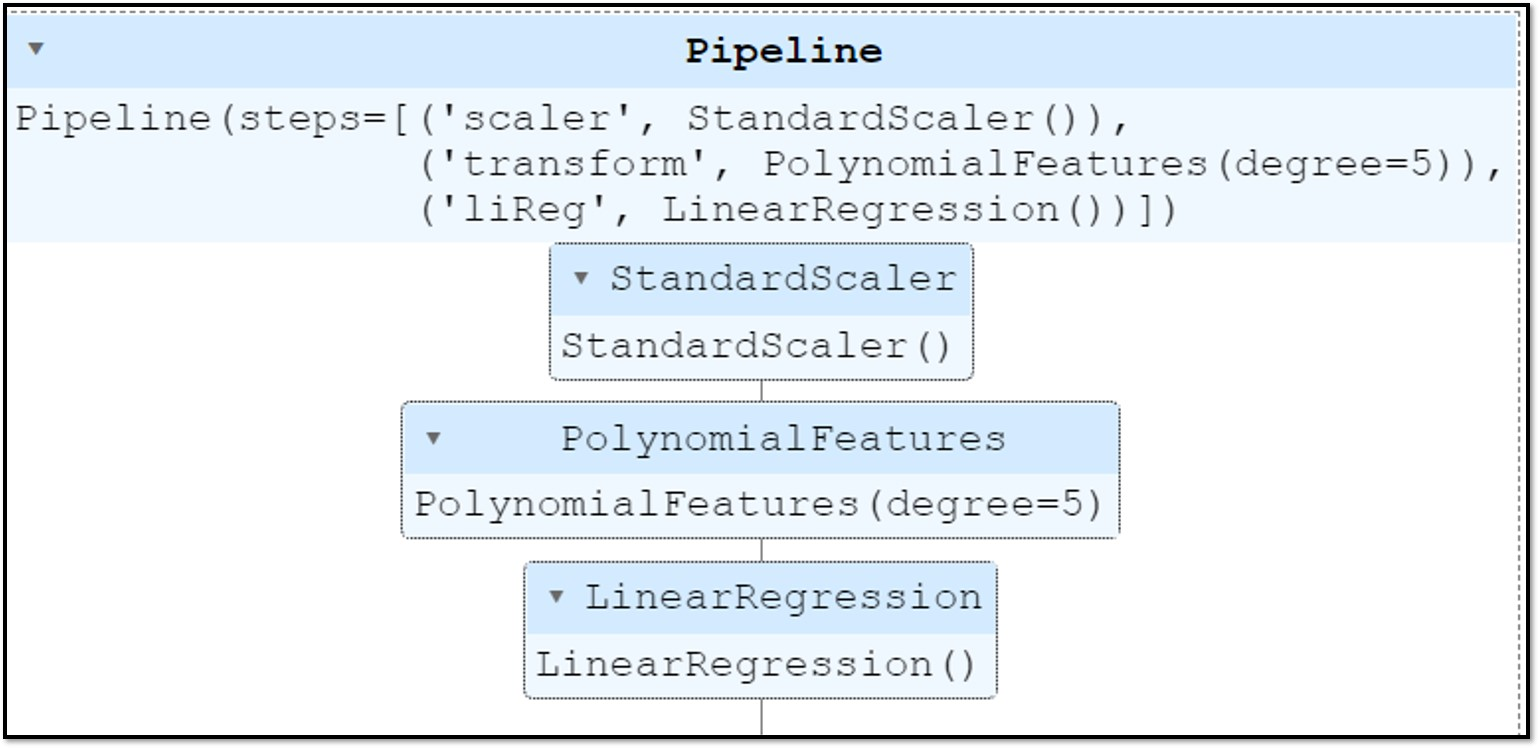
\includegraphics[width=8 cm]{pipeline.jpg}
  \caption{Pipeline for Modeling a Regression Model}
  \label{fig:pipeline}
\end{figure}

Figure \ref{fig:pipeline} summarizes the steps involved in implementing a regression model. The processes of feature scaling, polynomial transformation, and modeling can be done in one step by using the pipeline module in the sklearn library. This can make the process more efficient and organized, by chaining the different pre-processing and modeling steps together, and it can make it easy to try different combinations of pre-processing steps and models without having to repeat the same code over and over.

The following code demonstrates how to implement a polynomial regression model with a degree of 5 using the pipeline function. The pipeline function is used to combine the feature scaling using standardscaler function, polynomial transformation, and modeling steps into one step.

\begin{lstlisting}
# ==================================================#
from sklearn.pipeline import Pipeline

steps = [('scaler', StandardScaler()),
         ('poly', PolynomialFeatures(degree = 5)),
         ('liReg', LinearRegression())]

pipeline = Pipeline(steps)
pipeline.fit(X_train, y_train)
# ==================================================#
\end{lstlisting}

\newpage
\section{Performance Evaluation} \label{sec:evaluate}
This stage evaluates the predictive performance of the model using the test data set. There are different metrics to evaluate the model and the most common evaluation metrics are mean absolute error, mean squared error, and r2-score.

\subsection{Mean Absolute Error}

The mean absolute error (MAE) calculates how close the prediction is to the actual value on average and defines as:
\begin{equation}\label{mse}
  mae = \frac{1}{N} \sum_{i=1}^N |\tilde{y_i} - y_i|,
\end{equation}


\subsection{Mean Squared Error}
The mean squared error or root-mean squared error measures the average squared residuals (difference between the actual and the predicted values).
\begin{equation}\label{mse}
  mse = \frac{1}{N} \sum_{i=1}^N (\tilde{y_i} - y_i)^2,
\end{equation}

\begin{equation}\label{rmse}
  rmse = \sqrt{\frac{1}{N} \sum_{i=1}^N (\tilde{y_i} - y_i)^2},
\end{equation}

%MSE or RMSE is a good indicator to detect if the model predicted values that were significantly higher or lower than the actual values. If there is one or a few predicted values which are far away from the actual values, the mse or rmse will be significantly large compared to the mean absolute error.

\newpage
\subsection{R2-score}
R2 score, also known as the R-Squared score, is a metric that evaluates the goodness of fit of a regression model. It ranges from 0 to 1, with 1 indicating a perfect fit and 0 indicating a poor fit.
\begin{equation}\label{rmse}
  R^2 = 1- \frac{RSS}{TSS},
\end{equation} where $RSS$  is the sum of the squared differences between the predicted values and the actual values, while $TSS$ measures the total variance in the data by finding the sum of the squared differences between each data point and the average value. In other words, $TSS$ represents the total amount of variation in the data and $RSS$ represents the amount of variation that is not explained by the model. The definitions for $RSS$ and $TSS$ are as follows:

\begin{eqnarray}
% \nonumber to remove numbering (before each equation)$RSS$ 
  RSS &=& \sum_{i=1}^N (y_i-\tilde{y_i})^2 \\
  TSS &=& \sum_{i=1}^N (y_i-\bar{y_i})^2
\end{eqnarray} where $\tilde{y_i}$ is the predicted value and $\bar{y_i}$ is the mean value of the variable. 

The table below illustrates the calculation of $RSS$, $TSS$ and $R^2$ values in two extreme cases where $R^2=1$ and $R^2=0$.

\subsubsection{\textbf{Case 1: $R^2 = 1$}}
The first table demonstrates the first case when $R^2 = 1$. The predicted values are identical to the actual values, resulting in an $RSS$ value of zero. This scenario leads to an R2 score of 1, indicating a perfect fit of the data to the regression model. 

\begin{table}[h]
\centering
\begin{tabular}{|c|c|c|c| }
  \hline
  $y_i$ & $\tilde{y_i}$ & $(y_i-\tilde{y_i})^2$ & $(y_i-\bar{y_i})^2$  \\
  \hline
  10 & 10 & 0 & 100\\
  20 & 20 & 0 & 0\\
  30 & 30 & 0 & 100\\
  \hline
  $\bar{y_i}=20$ &  & RSS = 0  &  TSS = 200\\
  \hline
\end{tabular}
\caption{\textbf{Case 1}: Predicted and Actual Values are the same.}\label{tb:r2Case1}
\end{table}

\subsubsection{\textbf{Case 2: $R^2 = 0$}}
\begin{table}[h]
\centering
\begin{tabular}{|c|c|c|c| }
  \hline
  $y_i$ & $\tilde{y_i}$ & $(y_i-\tilde{y_i})^2$ & $(y_i-\bar{y_i})^2$  \\
  \hline
  10 & 20 & 100 & 100\\
  20 & 20 & 0 & 0\\
  30 & 20 & 100 & 100\\
  \hline
  $\bar{y_i}=20$ &  & RSS = 200  &  TSS = 200\\
  \hline
\end{tabular}
\caption{\textbf{Case 2}: Model always returns the average as predicted value.}\label{tb:r2Case2}
\end{table}

The second table illustrates the scenario where $R^2$  is 0, indicating a poor fit of the data to the regression model. In this case, the model always returns the average value of the actual data as the predicted value, resulting in an$RSS$ and $TSS$ value that are the same. This leads to an $R^2$ score of zero. 

It can be seen from these two examples that the R2 score ranges between 0 and 1, with a higher value indicating a better performance of the model. However, it's possible for the R2 score to be negative if the trained model performs worse than the baseline model which is returning the average values

It's worth mentioning that there is a variation of the R2 score called the adjusted R2 score, which takes into account the number of independent variables in the model. This metric helps in identifying irrelevant features in the model. However, the calculation of the adjusted R2 score is not covered in this book.

\newpage
\subsection{Implementation using Python}
The Python sklearn library offers a metrics module that can be used to compute various evaluation metrics for a model, such as R2 score. The functions in this module require the input of both the actual and predicted values. The predicted values can be obtained by using the 'predict' function of a trained model.

It is important to note that if any pre-processing steps were applied to the training data, such as feature scaling or polynomial transformation, the same pre-processing steps must be applied to the test data before using the model for evaluation. Failure to do so can result in a mismatch of feature spaces and negatively impact the model's performance.

However, it is crucial to ensure that the pre-processing parameters are only learned from the training data, and not from the test data. If information from the test data is used while building the model, it may appear to perform well on the test data but fail to perform well during actual deployment. This is known as "data leakage" problem, and it is crucial to avoid using any information from the test data while performing pre-processing steps to avoid such issues.

\subsubsection{\textbf{Evaluating the Linear Model}}
The code below demonstrates how to evaluate the multiple linear model that was previously trained. As the features were scaled using the standard scaler during training, it is necessary to scale the test data in the same way. The same mean and variance values used to transform the training data should be used to transform the test data, rather than learning new parameters from the test data set. 

In the sklearn library, this can be done by calling the 'transform' function during testing, as opposed to the 'fit\_transform' function used during training.

\begin{lstlisting}
# ==================================================#
from sklearn.metrics import mean_absolute_error
from sklearn.metrics import mean_squared_error
from sklearn.metrics import r2_score

X_test_scaled = scale.transform(X_test)
ytest_pred = lr.predict(X_test_scaled)

mae = mean_absolute_error(y_test, ytest_pred)
mse = mean_squared_error(y_test, ytest_pred,
                        squared= True)
r2 = r2_score(y_test, ytest_pred)
# ==================================================#
\end{lstlisting}
The root mean squared error (rmse) can be computed by setting the parameter \textbf{'squared'} to False.

\subsubsection{\textbf{Evaluating the Polynomial Model}}
When working with a polynomial regression model, it's important to remember that the same pre-processing steps used during training should be applied to the data before making predictions. In this case, the features were scaled using the standard scaler, and were also transformed using a fifth-order polynomial transform. Therefore, the same scaling and polynomial transformation steps should be applied to the data before making predictions with the model.

The code snippet below illustrates how to evaluate a polynomial regression model using a new test dataset in Python:

\begin{lstlisting}
# ==================================================#
from sklearn.metrics import mean_absolute_error
from sklearn.metrics import mean_squared_error
from sklearn.metrics import r2_score

X_test_scaled = scale.transform(X_test)
X_test_poly = poly.transform(X_test_scaled)
ytest_pred = lr_poly.predict(X_test_poly)

mae = mean_absolute_error(y_test, ytest_pred)
mse = mean_squared_error(y_test, ytest_pred,
                         squared= True)
r2 = r2_score(y_test, ytest_pred)
# ==================================================#
\end{lstlisting}


\subsubsection{\textbf{Evaluating the Pipeline}}

The sklearn library offers a "pipeline" function that can be used to prevent data leakage by ensuring that the appropriate pre-processing steps are applied to the correct data subset. With this function, it is not necessary to perform pre-processing steps separately, as the pipeline function takes care of it.

\begin{lstlisting}
# ==================================================#
from sklearn.metrics import mean_absolute_error
from sklearn.metrics import mean_squared_error
from sklearn.metrics import r2_score

ytest_pred = pipeline.predict(X_test)

mae = mean_absolute_error(y_test, ytest_pred)
mse = mean_squared_error(y_test, ytest_pred,
                        squared= True)
r2 = r2_score(y_test, ytest_pred)
# ==================================================#
\end{lstlisting}

\newpage
\subsection{Cross-Validation} \label{sec:cv}
Cross-validation is a technique that utilizes multiple test data sets to evaluate a model's performance, providing a more accurate idea of how the model will perform with new data. This is accomplished by first dividing the initial training data set into k subsets, known as folds. The model is then trained repetitively using k-1 subsets and tested on the remaining fold. This process is repeated until all folds have been used for testing. The model's performance is then evaluated for all folds and the average performance is reported.

The code below demonstrates how to use the Python sklearn "model\_selection" module to train a cross-validated polynomial regression model, making use of the pipeline function to avoid data leakage problems.

\begin{lstlisting}
# ==================================================#
from sklearn.model_selection import KFold
from sklearn.model_selection import cross_val_score

kfold = KFold(n_splits=5,shuffle=False)
steps = [('scaler', StandardScaler()),
         ('poly', PolynomialFeatures(degree = 4,
                                include_bias=False)),
         ('liReg', LinearRegression())]

pipeline = Pipeline(steps)
mse = -1*cross_val_score(pipeline, X_train, y_train,
                scoring = 'neg_mean_squared_error',
                cv=kfold)

print('average mean squared error is', np.mean(mse))
# ==================================================#
\end{lstlisting} The "KFold" function in the code snippet has a parameter named "n\_splits", which defines the number of subsets to be created, while the "cross\_val\_score" function provides a score (defined by the "scoring" parameter) for each fold. 

In this example, the number of splits is set to 5 and the scoring parameter is defined as negative mean squared error. This cross-validation method can also be used to optimize the hyper-parameters of a model using a grid search method, which will be covered in section \ref{sec:hyperP}.

\newpage
\subsection{Bias and Variance Trade-off}

The bias-variance trade-off is a fundamental concept in assessing the performance of supervised machine learning models.

\subsubsection{\textbf{Bias}}
Bias refers to the difference between a model's average prediction and the true value, and models that over-simplify and generalize relationships between variables fails to capture the actual trend in the data and tend to have a high bias. Simple linear regression models tend to have high bias and under-fit the data, resulting in large errors for both training and testing sets.

\subsubsection{\textbf{Variance}}
Variance measures how much the accuracy of a machine learning model can vary depending on the data set. It's common for a model to perform well on the training set but poorly on new or test data, which often occurs due to training on a small data set or over-fitting the training data, resulting in a loss of generalization.

\subsubsection{\textbf{Bias Variance Trade-off}}
\begin{figure}[!ht]
  \centering
  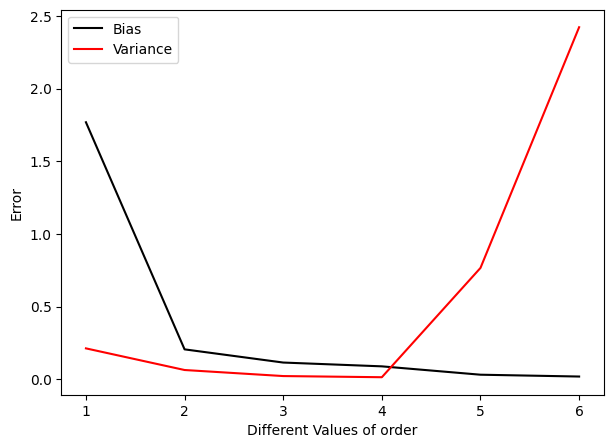
\includegraphics[width=8 cm]{Bias_Variance.png}
  \caption{Error vs. Order of regression model}
  \label{fig:bias_vari}
\end{figure}

Figure \ref{fig:bias_vari} illustrates how the model in the sales prediction example performs in relation to the order of the polynomial regression model. The error for the training data set (bias) decreases as the order of the polynomial regression model increases (i.e. the model becomes more complex), but the variance (difference in performance between training and testing data sets) increases with increasing model complexity.

A machine learning model should have an appropriate balance between bias and variance to avoid overfitting or underfitting the problem. In this example, the optimal result is achieved at order 4.


\newpage
\section{Regularization}\label{sec:regularization}

Regularization is a method to reduce over-fitting, particularly when there is a large variance between the train and test set performance. Regularization commonly achieved by modifying the loss function by adding a regularization term. This section will cover two popular regularization techniques: Lasso and Ridge Regression.

\subsection{Lasso Regression}
Lasso regression, also referred to as L1 regularization, is a technique that adds a penalty term based on the absolute value of the coefficient magnitude to the loss function.

\begin{equation}\label{eq:Lassocost}
  \varepsilon = \frac{1}{N}\sum_{i=1}^N (\tilde{y_i}-y_i)^2 + \alpha \sum_{j = 1}^{N_p} \parallel \omega_j \parallel,
\end{equation} where $N$ is the number of data points and $\tilde{y_i}$ is the predicted value using the model, $N_p$ is the number of parameters, $\omega_j, j = 1, 2, ..., N_p$ are parameters of the model and the parameter $\alpha$ controls the amount of regularization.

The parameter $\alpha$ reduces the value of coefficients and when it's sufficiently large, some of the coefficients $\omega_i$ will be eliminated. Therefore, Lasso regression is particularly useful when the model is suffering from multi-collinearity or when working with high dimensional data (number of features is more than the number of observations) and wanting to remove some of the less important features automatically.


\subsection{Ridge Regression}
Ridge regression is similar to Lasso regression, but instead of adding an $L1$ penalty term it adds an $L2$ norm penalty term to the loss function.

\begin{equation}\label{eq:ridgecost}
  \varepsilon = \frac{1}{N}\sum_{i=1}^N (\tilde{y_i}-y_i)^2 + \alpha \sum_{j = 1}^{N_p} \omega_j ^2,
\end{equation} where $N$ is the number of data points and $\tilde{y_i}$ is the predicted value using the model, $N_p$ is the number of parameters, $\omega_j, j = 1, 2, ..., N_p$ are parameters of the model and the parameter $\alpha$ controls the amount of regularization.

Unlike Lasso, Ridge regression never eliminates coefficients and thus, can't be used for automatic feature selection.

\newpage
\subsection{Lasso vs. Ridge}
In the example of predicting sales amount, three advertisement programs were used to predict the sale amount and the multiple linear regression model is represented as:

\begin{equation}\label{eq:polyResult}
  y = 3.893 x_1 + 3.420 x_2 + 2.943 x_3 + 13.788,
\end{equation} where $x_i$ are independent features. It can be observed that the variable $x_1$ is the most significant feature and has the highest coefficient.

\begin{table}[!ht]
\centering
\begin{tabular}{|c|r|r|r|r|}
  \hline
               & $\alpha = 0$  & $\alpha = 0.5$ & $\alpha = 1$ & $\alpha = 10$ \\
  \hline
  $\omega_1$ (L) & 3.893 & 3.420 & 2.943 & 0 \\
  $\omega_2$ (L) & 2.761 & 2.310 & 1.832 & 0 \\
  $\omega_3$ (L) & 0.067 & 0 & 0 & 0 \\
  \hline
  \hline
  $\omega_1$ (R) & 3.893 & 3.879 & 3.865 & 3.625 \\
  $\omega_2$ (R) & 2.761 & 2.749 & 2.738 & 2.546 \\
  $\omega_3$ (R) & 0.067 & 0.072 & 0.078 & 0.163 \\
  \hline
  \hline
\end{tabular}
\caption{Effects of the regularized parameter $\alpha$  on the Parameters}\label{tb:regular}
\end{table}

In this section, the model from the previous example of sales amount prediction is re-implemented using Ridge and Lasso regression with various regularization weights.

Table \ref{tb:regular} illustrates the effect of the regularization parameter $\alpha$ on the magnitude of coefficients in the Lasso and Ridge models. It is important to note that this implementation is only done to demonstrate the effect of the regularization parameter and regularization is not needed for this problem.

As we can see, Lasso regression eliminates coefficients for the least important variable $x_3$ when the parameter $\alpha$ becomes sufficiently large ($\alpha \geq 10$), while Ridge regression reduces the magnitude of high coefficients but keeps lower coefficient values.

\newpage
\section{Hyper-Parameter Tuning}\label{sec:hyperP}
Hyper-parameters are parameters that are set before modeling begins. Examples of typical parameters for a regression model include the order of a polynomial regression model, $k$, and the regularization parameter $\alpha$ in Lasso and Ridge models. The cross-validation method discussed in section \ref{sec:cv} is often used to find the best hyper-parameters for a machine learning model. These parameters are then used to develop a model that is deployed and tested on an initial testing data-set.

Grid search and random search are common methods for finding the best hyper-parameters for a model. These methods define a parameter space that includes a set of possible hyper-parameter values that can be used to build the model. Grid search method uses every combination of hyper-parameter values to train the model and select the best hyper-parameter. Random search method randomly selects and tests a random combination of hyper-parameters and it is more efficient than grid search for a higher number of parameters. 

The code below shows an example of how to find the hyper-parameter $k$ for a polynomial regression model using the Grid search method.


\newpage

\begin{lstlisting}
# ==================================================#
from sklearn.model_selection import GridSearchCV

steps = [('scaler', StandardScaler()),
         ('poly', PolynomialFeatures(degree = order,
                                include_bias=False)),
         ('liReg', LinearRegression())]
parameters = {"poly__degree":[1, 4, 6, 9]}
pipeline = Pipeline(steps)

poly_grid = GridSearchCV(pipeline, parameters,
                         cv=4,
                        scoring='neg_mean_squared_error')

poly_grid.fit(X_train, y_train)
print ('best order is :', poly_grid.best_params_)

y_pred_test = poly_grid.predict(X_test)
mae = mean_absolute_error(y_test, y_pred_test)
# ==================================================#
\end{lstlisting}



\newpage
\section{Project: Sale Amount Prediction}\label{sec:LRproject1}

A complete example for predicting the sale amount based on different advertisement programs is provided below. The data set used in this example is small, containing four features and 200 rows of entries. The "sale amount" is the target feature, and the other three features are the costs associated with the "TV", "radio", and "newspaper" programs. The data set can be downloaded from the provided \href{https://www.kaggle.com/sazid28/advertising.csv}{link}\cite{web:adData}. Note that the data has already been cleaned and no missing data is present.

\subsection{Data Importing}
The initial step is to import the required modules and then read the data from the computer.

\begin{lstlisting}
# ==================================================#
import pandas as pd

df=pd.read_csv('..\\data\Advertising.csv')

X=df[['TV', 'radio', 'newspaper']].values
y=df['sales'].values

# ==================================================#
\end{lstlisting}

\newpage
\subsection{Train-Test-Split}
The data is divided into training and testing data sets. Two-thirds of the data is allocated for training, and the remaining one-third is reserved for testing.
\begin{lstlisting}
# ==================================================#
from sklearn.model_selection import train_test_split

X_train, X_test, y_train, y_test = train_test_split(X,y,
                                    test_size = 0.33,
                                    random_state=1)
# ==================================================#
\end{lstlisting}

\newpage
\subsection{Modeling and Hyper-Parameter Tuning}
The grid search method is applied to determine the hyper-parameter $k$, which is the order of the polynomial regression model. The pipeline function is utilized to prevent potential data leakage issues.

\begin{lstlisting}
# ==================================================#
from sklearn.model_selection import GridSearchCV
from sklearn.preprocessing import StandardScaler
from sklearn.preprocessing import PolynomialFeatures
from sklearn.linear_model import LinearRegression
from sklearn.pipeline import Pipeline

steps = [('scaler', StandardScaler()),
         ('poly', PolynomialFeatures(degree = 2,
                                include_bias=False)),
         ('liReg', LinearRegression())]
parameters = {"poly__degree":[2, 3, 4, 5, 7, 9]}
pipeline = Pipeline(steps)
poly_grid = GridSearchCV(pipeline, parameters,
                         cv=5,
                        scoring='neg_mean_squared_error',
                        verbose= True)
poly_grid.fit(X_train, y_train)
print ('best order is :', poly_grid.best_params_)
# ==================================================#
\end{lstlisting}

\newpage
\subsection{Model Evaluation}
The performance of the best model is evaluated on both the training and testing data sets.

\begin{lstlisting}
# ==================================================#
rom sklearn.metrics import mean_absolute_error
from sklearn.metrics import mean_squared_error
from sklearn.metrics import r2_score

# Evaluation on the Tesing data set
ytest_pred = poly_grid.predict(X_test)
mae = mean_absolute_error(y_test, ytest_pred)
mse = mean_squared_error(y_test, ytest_pred,
                        squared= True)
r2 = r2_score(y_test, ytest_pred)
#Evaluation on the Training data set
ytr_pred = poly_grid.predict(X_train)
maeT = mean_absolute_error(y_train, ytr_pred)
mseT = mean_squared_error(y_train, ytr_pred,
                        squared= True)
r2T = r2_score(y_train, ytr_pred)
#Keep all results in the tabular form
result = pd.DataFrame({'mae': [maeT, mae],
                        'mse': [mseT, mse],
                        'r2': [r2T, r2]})
result.index = ['Training', 'Testing']
# ==================================================#
\end{lstlisting}

It is suggested that readers download the full codes and data sets from the public \href{https://github.com/myothida/Intro-To-Supervised-Machine-Learning.git}{\textbf{GitHub Repo}} and experiment with running the code using different data sets.
